%
% 
%
% Contact: konvens2018@oeaw.ac.at
%%
%% Based on the style files for KONVENS 2016, which were, in turn,
%% Based on the style files for GSCL-2015, which were, in turn,
%% Based on the style files for ACL-2014, which were, in turn,
%% Based on the style files for ACL-2013, which were, in turn,
%% Based on the style files for ACL-2012, which were, in turn,
%% based on the style files for ACL-2011, which were, in turn,
%% based on the style files for ACL-2010, which were, in turn,
%% based on the style files for ACL-IJCNLP-2009, which were, in turn,
%% based on the style files for EACL-2009 and IJCNLP-2008...

\documentclass[11pt]{article}
\usepackage{konvens2018}
\usepackage{mathptmx}
\usepackage[scaled=.90]{helvet}
\usepackage{courier}
\usepackage{xcolor}
\usepackage{url}
\usepackage{latexsym}
\usepackage{tipa}
\usepackage{enumitem}
\usepackage{csquotes}

\usepackage{graphicx}
\usepackage{caption}
\usepackage{subcaption}

\usepackage{makecell}

%\usepackage{hyperref}
\def\UrlBreaks{\do\/\do-}

% import acronyms
\usepackage[nolist]{acronym}

\usepackage{booktabs}

%\usepackage{textcomp}

%\setlength\titlebox{5cm}

% You can expand the titlebox if you need extra space
% to show all the authors. Please do not make the titlebox
% smaller than 5cm (the original size); we will check this
% in the camera-ready version and ask you to change it back.


\title{KAUSTmine - Offensive Comment Classification on German Language Microposts}

\author{Matthias Bachfischer\thanks{\tt \space bachfischer.matthias@googlemail.com} \qquad Uchenna Akujuobi \thanks{\tt  \space uchenna.akujuobi@kaust.edu.sa} \qquad Xiangliang Zhang\thanks{\tt  \space xiangliang.zhang@kaust.edu.sa} \\
   Computer, Electrical and Mathematical Sciences and Engineering Division \\
     King Abdullah University for Science and Technology (KAUST) \\
}
  
\date{}

\begin{document}

\begin{acronym}[\hspace{1.8cm}]
\acro{auc}[AUC]{Area Under Curve}
\acro{cnn}[CNN]{Convolutional Neural Network}
\acro{lstm}[LSTM]{Long Short-Term Memory}
 \acro{nlp}[NLP]{Natural Language Processing}
 \acro{nn}[NN]{Neural Network}
 \acro{url}[URL]{Uniform Resource Locator}
 \acro{relu}[RELU]{Rectified Linear Unit}
 \acro{roc}[ROC]{Receiver Operating Characteristic}
 \acro{sgd}[SGD]{Stochastic Gradient Descent}
\acro{svm}[SVM]{Support Vector Machine}
\acro{tf-idf}[TF-IDF]{Term-Frequency times Inverse Document-Frequency}

\end{acronym}

\maketitle
\begin{abstract}
In this paper, we present two deep-learning based classifier systems for the identification of offensive comments in German Language microposts: A bidirectional LSTM and a CNN model. We compare the performance of our systems with a traditional, machine-learning based SVM classifier and evaluate our approach on Task 1 (binary classification) of the GermEval 2018 shared task where our best model (CNN) is able to reach a F1 score of 91.08\%.
\end{abstract}

\nocite{RN65}

\section{Introduction}
Modern communication devices and social media play an increasingly important role in our daily lives and the Internet has created tremendous opportunities for exchanging information with people from all over the globe in real-time. Unfortunately however, this freedom gets frequently abused, and hate speech and toxic comments are present in virtually all online communities. A 2017 report by Pew Research even came to the conclusion that up to 41\% of all adults have personally experienced online harassment \cite{RN63}.
\newline
Automated detection routines to identify and block toxic messages have proven to be viable methods in shielding online communities from harassment \cite{RN27}. Training a computer to understand the emotions and opinions expressed in a document is a common task in the area of \ac{nlp}, and the results from previous publications  \cite{RN14} as well as a Kaggle competition \footnote{Toxic Comment Classification Challenge \url{https://www.kaggle.com/c/jigsaw-toxic-comment-classification-challenge}} sponsored by Google Jigsaw have already shown promising results for the identification of toxic content in online messages.
\newline
The intention of this paper at hand is to create a series of deep-learning based neural network models to compete in Task 1 (binary classification) of the GermEval 2018\footnote{\label{footnote:germ2018}Germeval 2018 - Shared Task on the Identification of Offensive Language - \url{https://projects.cai.fbi.h-da.de/iggsa}} competition. The GermEval 2018 competition is a shared task for the identification of offensive comments in German language microposts. For our research, we choose a simple \ac{svm} model as a baseline and compare its performance against our implementations of a bidirectional \ac{lstm} and a \ac{cnn} model. 
\section{Related Works}
So far, most of the research in the area of toxic comment classification has been focused on English language, and a variety of machine-learning and deep-learning models have been produced to tackle this problem \cite{RN56}.  Amongst others, Georgakopoulos et al. \shortcite{RN14} used a deep-learning based \ac{cnn} model to detect toxic language in online content. Nobata et al. \shortcite{RN73}, on the other hand, developed a machine-learning model using a variety of feature classes (N-grams, Syntactic Semantics etc.) and were able to outperform existing deep-learning based approaches. Other research by Razavi et al. \shortcite{RN74} used multi-level classification to detect offensive comments, mainly in Usenet messages. 
\newline
The identification of toxicity in German language messages has received less attention by the research community so far, and comparable research results are sparse. In the related domain of sentiment analysis for tweets, Cieliebak et al. \shortcite{RN49} created a corpus consisting of 10.000 tweets in German language and provided benchmarks for the classification of these tweets into sentiment classes of either \textit{positive, negative} or \textit{neutral} using a \ac{cnn}.   

\section{Data}
\label{sec:data}
Before training our systems, we first obtain the training set from the GermEval 2018 competition mailing list. The training set contains a total of 5009 messages which have been labeled either \textit{OFFENSE} or \textit{OTHER}. A detailed breakdown of the class distribution in the dataset is presented in Table \ref{tbl:dataset}.
\begin{table}[h]
\begin{center}
\begin{tabular}{l c c c }
\toprule \bf Dataset &  Offense &  Other &  Total \\ \midrule
Training set & 1688 & 3321 & 5009 \\
\bottomrule
\end{tabular}
\end{center}
\caption{\label{tbl:dataset} Class distribution - GermEval 2018 dataset}
\end{table}
\newline
The dataset is imbalanced, and the majority of the tweets (66\%) belong to the neutral class, whereas the remaining data (34\%) belongs to the offensive class. The microposts within the dataset were extracted exclusively from Twitter\footnote{Twitter social network - \url{https://twitter.com}} because the conference organizers regarded tweets \enquote{as a prototypical type of micropost}\footnotemark[2].
\section{Experimental Setup}
We present two classification systems in our research: a bidirectional \ac{lstm} model and a \ac{cnn} model. Both models were implemented in Python and make use of the Keras library \cite{RN64} for training the classifier. In addition, we create a \ac{svm} classifier using Scikit-learn \cite{scikit-learn} and consider this as a baseline for testing and improving our deep-learning models. The experiments were performed on a workstation running Ubuntu 16.04 with 64 cores and 128 GB of RAM.
\newline
For this research we use the word vectors published by Deriu et al.\shortcite{RN62}. These vectors were trained on a total of 200 million tweets and have a dimensionality of $d=200$.
\newline
\textbf{Preprocessing: }
Before extracting features, we first preprocess the data according to the following procedure:
\begin{enumerate}[topsep=1.5pt,itemsep=-1ex,partopsep=1ex,parsep=1ex] 
  \item Replace URLs, usernames and retweets with replacement tokens \textit{URLTOK}, \textit{USRTOK} and \textit{rt}
  \item Convert tweet text to lowercase
  \item Convert categorical classification variables into an One-Hot encoded vector
  \item Tokenize tweets (using Keras's builtin Tokenizer) and create a list of word indexes with length $l=100$ (comments shorter than 100 are padded with 0)
\end{enumerate}
For further reference, a preprocessed tweet is presented in Example 4.1.
\newline
\noindent\fcolorbox{black}{gray!15}{
\begin{minipage}{0.95\columnwidth}
\textbf{Example 4.1:}
\newline
\textbf{Original:} \textit{@salzmanufaktur @Renft1964} Jetzt bekommt Merkel noch Gr\"une Untergangs-Beschleuniger dabei!
\newline
\textbf{Preprocessed:} \textit{USRTOK USRTOK} jetzt bekommt merkel noch gr\"une untergangs-beschleuniger dabei!
\end{minipage}}
\section{System Description}
After preprocessing, we feed the data into our classification models: a bidirectional \ac{lstm} and a \ac{cnn} model. By using the word vectors from Deriu et al., we create an embedding matrix where we randomly initialize the words that are not in the word embeddings with the arithmetic mean and standard deviation obtained from the embeddings. The resulting embedding matrix has the size of \textpipe $\vec{w_1}; ... ;\vec{w_L} \textpipe \in \rm{I\!R}^{L\times200}$ with $L$ being the number of unique words in our training set.
\newline
While training our models, we try to minimize the binary cross entropy loss on the training set given per the formula below:
\begin{equation}
-\frac{1}{N}\sum_{i=1}^N [y_i \log(\hat{y}_i)+(1-y_i) \log(1-\hat{y}_i)]
\end{equation}
The final outputs of the models are connected to a softmax regression layer which returns the class $\hat{y}\in[1,K]$ with the largest propability
\begin{equation}
{\displaystyle \hat{y}=\arg\max_{j} \ P(y=j\mid \mathbf {x} )={\frac {e^{\mathbf {x} ^{\mathsf {T}}\mathbf {w} _{j}}}{\sum _{k=1}^{K}e^{\mathbf {x} ^{\mathsf {T}}\mathbf {w} _{k}}}}}
\end{equation}
where $w_j$ denotes the weight vector for class $j$. For the optimization step, we choose the \textit{Adam} optimizer \cite{RN67} with a learning rate $lr=0.001$, $\beta_1=0.99$, $\beta_2=0.999$ and $\epsilon=1^{-8}$.
\subsection{LSTM Model}
\begin{figure*}
\centering
  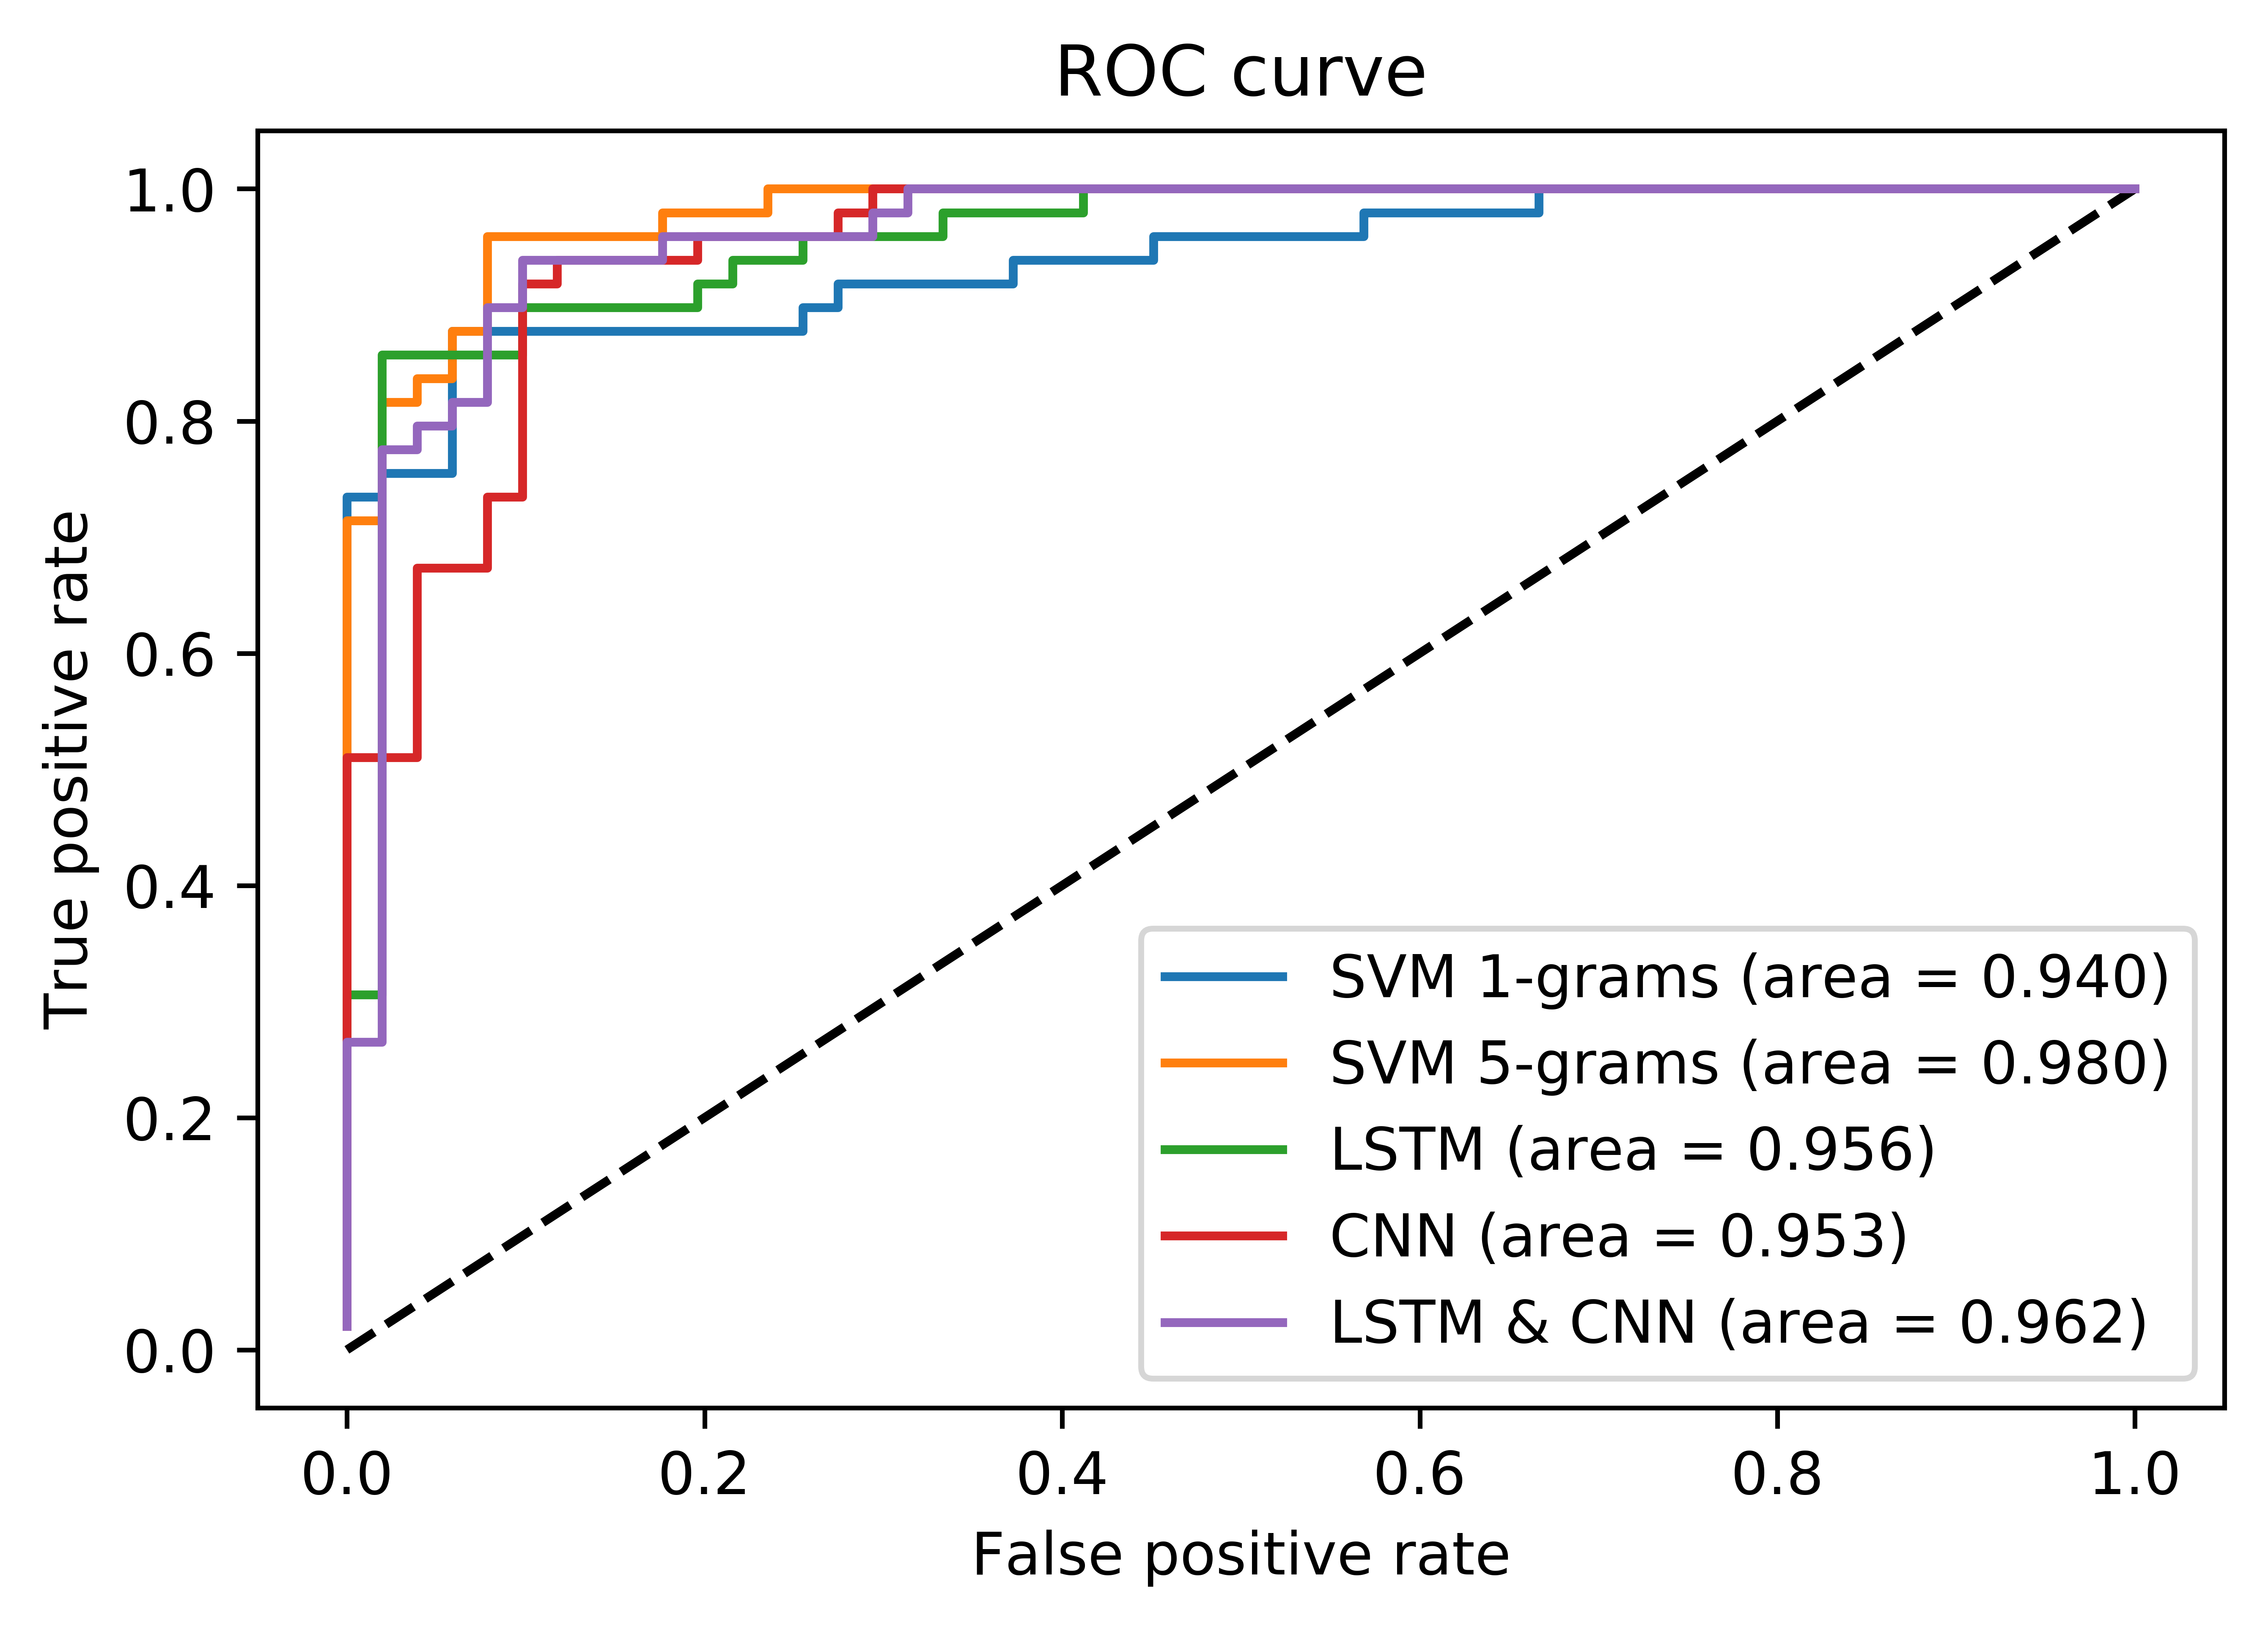
\includegraphics[width=0.8\linewidth]{roc_curve}
 \caption{Comparison of ROC metric for our models (PLACEHOLDER)}
\label{fig:f1_scores}
\end{figure*}
The \ac{lstm} model in this research was derived from the works of Hochreiter and Schmidhuber (1997). So far, \ac{lstm} networks have been successfully applied in a variety of tasks such as Machine Translation \cite{RN76} and Image Captioning \cite{RN77}. Recent research however shows that \ac{lstm} models also perform well when applied to \ac{nlp} tasks such as text classification \cite{RN57,RN78}.
\newline 
In this paper, we employ a bidirectional \ac{lstm} model with 64 units. The output is passed to two fully connected layers with 64 and 2 units respectively. To prevent our model from overfitting, we  apply the early-stopping technique \cite{RN79} in combination with a dropout of $d=0.5$ after the first dense layer as well as on the recurrent input signal of the \ac{lstm} units \cite{RN66}. We furthermore use \ac{relu} as the activation function of the first hidden layer \cite{RN71,RN72}. 
\subsection{CNN Model}
The \ac{cnn} model used in this research builds on the work of Kim \shortcite{RN35} who proposed to use a 2 layered \ac{cnn} to perform sentence classification in \ac{nlp} tasks. We create our model by using 1 convolutional layer with 64 filters (one layer consists of a convolution and a pooling layer). The output of the convolutional layers is then fed into one dense layer of 64 units.  As in the previous model, we again make use of the \ac{relu} function for the activation of the layer and apply early-stopping in combination with a dropout of $d=0.5$.
\subsection{Ensemble}
To further improve the overall performance, we create an ensemble by combining the results from the \ac{lstm} and the \ac{cnn} model. To create the ensemble, we average the probability outputs from both models and apply the $argmax$ function to obtain the binary outputs. We then use these predictions for the final submission run of the GermEval 2018 task.
\subsection{SVM Model}
As a baseline for the evaluation of our results, we use a simple \ac{svm} classifier trained on \ac{tf-idf} vectors \cite{RN75} of the tweets in the dataset. The \ac{tf-idf} scores were calculated by using the count matrices of 1-grams and 5-grams where the tweet texts serve as input tokens. The classifier uses \ac{sgd} with the logistic regression loss function where we multiply the regularization term with a constant $\alpha=1^{-5}$.
\section{Results}
\textit{Since the official test set will only be published by the task organizers on July 17, 2018, the authors of this paper used a sample set with size $n=100$ obtained from the conference website to conduct their preliminary experiments. Once the official test data is published, this section will be updated and the final results will be submitted to the shared task.} 
\newline
\newline
For the evaluation of our models, we use the script provided by the competition organizers to calculate the F1-score on the test set (size $n=100$). In Table \ref{tbl:results}, we present the F1-scores for each category. We further marked the best result in bold face. 
\newline
The \ac{cnn} model achieved best results on the given dataset (F1 score of 91.08), followed by the \ac{lstm} and \ac{svm} model using 5-grams (both reach a F1-score of 90.49). In comparison to that, the ensemble (with a F1-score of 88.46) performs poorly in comparison to the \ac{svm} classifiers. We consider this result surprising, since we were actually able to create pretty good classifiers by just calculating the \ac{tf-idf} vectors on n-grams obtained from the tweet texts. 
\newline 
\begin{table}[h]
\begin{center}
\begin{tabular}{l  c c c }
\toprule   &  Offense &  Other &   Average  \\ \midrule
SVM (1-grams) & 85.71 & 88.07 & 87.33  \\
SVM (5-grams) & 88.89 & 90.91 & 90.49  \\
LSTM & 88.89 & 90.91 & 90.49  \\
CNN & 91.09 & 90.01 & \textbf{91.08}  \\
LSTM \& CNN & 86.67 & 89.09 & 88.46  \\
\bottomrule
\end{tabular}
\end{center}
\caption{\label{tbl:results} F1-Scores per Category}
\end{table}
\newline
To evaluate the output of our classifiers, we further included a \ac{roc} curve metric in Figure 1 where we calculated the \ac{auc} score for each of our classifers. As we can see, the \ac{svm} model trained on 5-grams generally outperforms our collection of deep-learning based classifiers. The ensemble, created from the \ac{lstm} and \ac{cnn} classifiers, achieves the second-best \ac{auc} score, followed by the \ac{svm} where we used 1-grams.
\newline
Overall, and given the current excitement about the use of deep-learning based classifiers for \ac{nlp} tasks, we consider these results surprising. Even though we provided the \ac{svm} classifier with only one feature (\ac{tf-idf}), it was able to achieve very promising results and outperformed our deep-learning systems. 
\newline
\textit{Once the official test data is released, we will update this section with an in-depth discussion of the results.}
\section{Conclusion}
The objective of our participation in the GermEval 2018 shared task was to evaluate the performance of deep-learning based models on the classification of offensive language in German microposts. While using a \ac{svm} classifier as a baseline, we presented two deep-learning based systems and evaluated their results on the given dataset: a bidirectional \ac{lstm} model and a \ac{cnn} model. As a result from this research, we have shown that our \ac{cnn} model outperforms the \ac{lstm} model on the given GermEval dataset. 
%By combining the output of the \ac{lstm} and \ac{cnn} model in a single ensemble, we are able to reach a F1-score of 84.95\% in the final evaulation of the GermEval competition.
\newline
We hope that online social network platforms can use our results to build systems that can successfully detect and combat toxicity in online conversations. Services such as the Perspective API \footnote{Perspective API - \url{https://www.perspectiveapi.com/}} are taking a step into the right direction, and we expect to see more fascinating research for making the Internet a more friendlier and welcoming place.
% include your own bib file like this:
\bibliographystyle{konvens2018}
\bibliography{references.bib}


\end{document}
